\chapter{Formulazione}
\label{chap:formulazione}

\section{Definizione del problema }
\label{sec:problem}

Partendo da materiale testuale presente in rete, in particolare un dataset messo a disposizione da \emph{Yelp Dataset Challenge} contenente \numprint{5200000} reviews relative a \numprint{174000} business di 11 aree metropolitane nel mondo, l'obiettivo è quello di estrarre da questi dati caratteristiche di personalità.\\ 
Il nostro scopo è di identificare un adeguato spazio semantico che permetta di definire la personalità dell'oggetto target a cui un determinato testo si riferisce.

\section{Descrizione del dataset}
\label{sec:dataset}

Come punto di partenza, viene messo a disposizione un dizionario di 637 aggettivi, che la letteratura psicologica definisce come marker dei cinque grandi tratti di personalità noti come \emph{Big Five}.
In particolare, questo vocabolario associa ad ogni aggettivo un vettore di cinque elementi in cui ogni elemento corrisponde al grado di presenza o assenza di una determinata caratteristica.
\begin{figure}[H]
	\centering
\begin{tabular}{lccccc}
	\toprule
	 \textbf{Adjective} \quad & \multicolumn{5}{c}{\textbf{OCEAN}} \\
	
\midrule
	Active  & 0,053194 & 0,237406 & 0,365915 & 0,116700 & -0,058669  \\
	Angry  & -0,004604 & -0,038453 & 0,020755 & -0,294754 & 0,590114 \\
	Boring & -0,069877 & -0,099754 & -0,478821 & -0,236462 & 0,118821\\
	\rule{7pt}{0\normalbaselineskip} \dots &   \dots 		&			 \dots &			\dots &			 \dots & \dots \\
	\bottomrule
\end{tabular}
\captionof{table}{Esempio di dizionario OCEAN}
\label{tab:ocean}
\end{figure}

\section{Calcolo della Ground Truth}
\label{sec:GroundTruth}

Per poter addestrare correttamente il modello è necessario avere una Ground Truth, ovvero una label associata ad ogni input della rete. Senza questa informazione sarebbe impossibile ottimizzare il modello e valutarne la validità. 

Si procede eliminando dal dataset tutte le sentences non contenenti almeno uno degli aggettivi presenti nel dizionario OCEAN. In seguito verranno utilizzati i dati contenuti all'interno del vocabolario per creare una mappatura diretta tra ogni frase e il corrispondente vettore di personalità, in cui ogni elemento sarà calcolato come la media del valore di ogni aggettivo presente nel testo.

\section{Preprocessing}
\label{sec:preprocessing}
Gli algoritmi di apprendimento automatico non sono in grado funzionare direttamente con il testo non elaborato, è quindi necessario eseguire in primis un preprocessamento del database di testi e in seguito convertire i dati in numeri, nello specifico, in vettori di numeri.\\
Alla fine di questo processo il dataset ottenuto sarà suddiviso in tre corpora: 
\begin{itemize}
	\item $70\%$ training set : contenente \numprint{4351900} reviews utilizzate dalla rete per l'apprendimento;
	\item $10\%$ validation set: contenente \numprint{621700} reviews;
	\item $20\%$ testing set: contenente \numprint{1243000} reviews.
\end{itemize}
La divisione dei tre dataset dovrà mantenere una buona distribuzione fra le diverse classi.

\subsection{Natural Language Processing}
\label{subsec:nlp}
Il \emph{Natural Language Processing} (NLP) è un insieme di tecniche di computer science e linguistica che ricorrono a dei calcolatori per analizzare il linguaggio umano.
\\

Dal punto di vista sintattico, al dataset viene applicata la seguente serie di operazioni:
\begin{itemize}
	\item \textbf{Rottura della frase}: dato un pezzo di testo vengono trovati i limiti della frase, spesso contrassegnati da punti o altri segni di punteggiatura.
	\item \textbf{Stemming}: alcune parole vengono ridotte alla loro forma radice (ad esempio ``argue, argued, argues, arguing, and argus'' sono mappati alla parola ``argu'').
	\item \textbf{Segmentazione di parole}: un blocco di testo o sentence viene separato in parole. Per una lingua come l'inglese, questo è abbastanza banale, poiché le parole sono solitamente separate da spazi. 
\end{itemize}
Dal punto di vista semantico invece si interviene nel seguente modo:
\begin{itemize}
	\item \textbf{Semantica lessicale}: tenta di comprendere il significato computazionale delle singole parole nel loro contesto.
	\item \textbf{Comprensione del linguaggio naturale}: i blocchi di testo vengono convertiti in rappresentazioni più formali e più facili da manipolare per i computer. 
\end{itemize}
Ricorrendo, dove possibile, alle tecniche sopraelencate, è possibile costruire un dizionario delle \numprint{60000} parole più frequenti nel corpus di training, basato sulla frequenza assoluta di una parola, avendo cura di eliminare tutti gli aggettivi presenti nel dataset OCEAN.

\begin{figure}[H]
	\centering
	{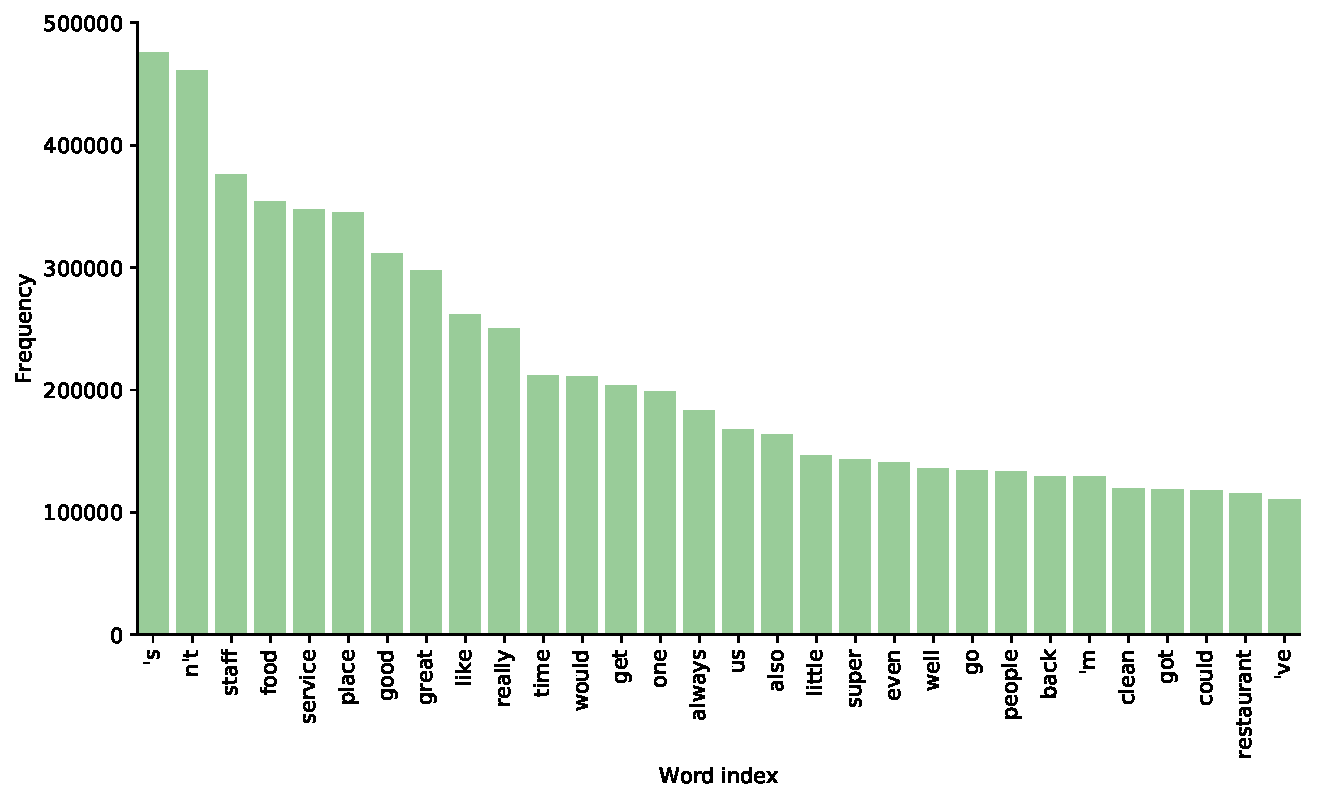
\includegraphics[width=.8\textwidth]{images/dict_histogram30}}
	\caption{Istogramma rappresentativo delle 30 parole più frequenti nel dizionario}
	\label{fig:Istrogramma del dizionario}
\end{figure}
In questo modo non verrà influenzata la rete mostrando l'associazione tra gli aggettivi e le label associate, ed il modello sarà ``costretto'' ad imparare il legame esistente tra il contesto di una frase e il relativo valore del tratto di personalità. 

Inoltre sarà necessario anche rimuovere tutte le \emph{stopwords} relative alla lingua inglese, ovvero parole considerate poco significative perché usate troppo frequentemente all'interno delle frasi --- per esempio gli articoli e le congiunzioni --- filtrando i termini comuni e senza uno specifico significato semantico dalle parole che trasportano vere informazioni.

In seguito ogni parola del dizionario verrà codificata con un valore intero univoco, mentre quelle non presenti, tra cui gli aggettivi mappati nel vocabolario OCEAN, verranno indicizzati al valore ``-1'' e gli verrà associato il token ``UNK'' come mostrato nella Figura~\ref{fig:preprocessing}
\begin{figure}[H]
	\centering
	{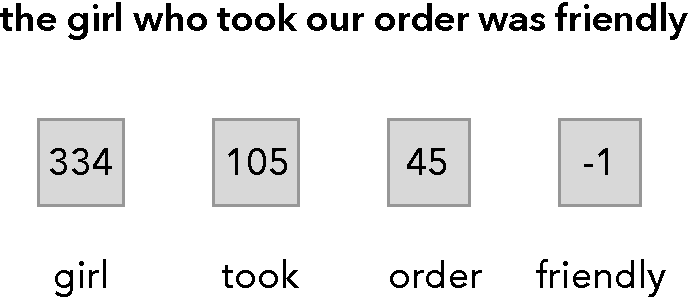
\includegraphics[width=.5\textwidth]{images/preprocessing}}
	\caption{Visualizzazione del preprocessing}
	\label{fig:preprocessing}
\end{figure}

